\documentclass{./llncs2e/llncs}
% \usepackage[printonlyused]{acronym} 
\usepackage{graphicx}
\usepackage{fixltx2e}
\usepackage{mathtools}
\usepackage[nolist,nohyperlinks]{acronym}
% \addtolength\textwidth{3cm}
\usepackage[margin=2.9cm]{geometry}
% 
% Title 
% 

\begin{document}
\title{browserCloud.js}
\titlerunning{browserCloud.js}
\toctitle{browserCloud.js}

\subtitle{A federated community cloud served by a P2P overlay network on top of the web platform}
\author{David Dias, david.dias@computer.org}
\authorrunning{David Dias}
\tocauthor{David Dias}
\institute{Lisbon Tech, University of Lisbon}

\maketitle

%!TEX root = ../index.tex

% 
% Abstract 
% 

\begin{abstract}
Grid computing has been around since the 90's, its fundamental basis is to use idle resources in geographically distributed systems in order to maximize its efficiency, giving researchers access to computational resources to perform their jobs (e.g. studies, simulations, rendering, data processing, etc). This approach quickly grew into non grid environments, causing the appearance of projects such as SETI@Home or Folding@Home, that use volunteered shared resources and not only institution-wide data centers as before, creating the concept of Public Computing. Today, after having volunteering computing as a proven concept, we face the challenge of how to create a simple, effective, way for people to participate in this community efforts and even more importantly, how to reduce the friction of adoption by the developers and researchers to use this resources for their applications. This work explores current ways of making an interopable way of end user machines to communicate, using new Web technologies, creating a simple API that is familiar to those used to develop applications for the Cloud, but with resources provided by a community and not by a company or institution.

\end{abstract}
%!TEX root = ../index.tex

% 
% Keywords 
% 

\begin{keywords}
Cloud Computing, Peer-to-peer, Voluntary Computing, Cycle Sharing, Decentralized Distributed Systems, Web Platform, Javascript, Fault Tolerance, Reputation Mechanism, Community Cloud.
\end{keywords}
%!TEX root = ../index.tex

% 
% Introduction
% 

\section{Introduction}

Cloud computing has revolutionized the computing landscape mainly due to key advantages to developers/users over pre-existing computing paradigms, the main reasons are:
\begin{itemize}
  \item Virtually unlimited scalability of resources, avoiding disruptive infrastructure replacements.
  \item Utility-inspired pay-as-you-go and self-service purchasing model, minimizing capital expenditure
  \item Virtualization-enabled seamless usage and easier programming interfaces
  \item Simple, portable internet service- based interfaces, straightforward for non expert users, enabling adoption and use of cloud services without any prior training
 \end{itemize} 

Grid computing had offered before a solution for high CPU bound computations, however it has high entry barriers, being necessary to have a large infrastructure, even if just to execute small or medium size computing jobs. Cloud computing solves this by offering a solution ``pay-as-you-go'', which transformed computing into an utility.

Still, even though we are able to integrate several Cloud providers into an open software stack, Cloud computing relies nowadays on centralized architectures, using mainly the Client-Server model. This work pursues a shift in this paradigm.

Unlike the conventional approach to make Cloud Computing `green' (i.e. Green Computing) by improving datacenter's efficiency through expensive and strictly centralized control, our vision entails a shift in perspective, by enabling each user to contribute to this effort, by leveraging his/her idle computing resources (sometimes up to 70\% of power wasted), and thus reducing overall environmental footprint. Thus browserCloud.js resources are provided in a voluntary manner by common Internet users that want to share their idle computer cycles and storage available, while browsing the web, without having the concern to setup any application or system to do so.

Community Clouds are not a novelty in the Distributed Systems research area. However, existing models have been developed to follow the client-server model, transporting the data to the place where the computation will take place, which causes big bottlenecks in network traffic, limiting the amount of computed units done in a delimited window of time. One of browserCloud.js goals is exactly to mitigate this bottleneck by taking the computation (the algorithms that will perform operations over the data) to the machines where the data is stored.

To accomplish this, we propose a new approach to abandon the classic centralized Cloud Computing paradigm, towards a common, dynamic, and privacy-aware cloud infrastructure. This, by means of a fully decentralized architecture, federating freely ad-hoc distributed and heterogeneous resources, with instant effective resource usage and progress. Additional goals may include: arbitration, service-level agreements, resource handover, compatibility and maximization of host's and user's criteria, and cost- and carbon-efficiency models.

The work will address extending the Web Platform with technologies such as: WebRTC, Emscripten, Javascript and IndexedDB to create a structured peer-to-peer overlay network, federating ad-hoc personal resources into a geo-distributed cloud infrastructure, representing the definition made by C.Shirky of what an peer-to-peer means:

  \textit{``An application is peer-to-peer if it aggregates resources at the network’s edge, and those resources can be anything. It can be content, it can be cycles, it can be storage space, it can be human presence.''}, C.Shirky \cite{Shirky.}

Finally, browserCloud.js has the possibility to grow organically with the number of users. The management of this resources is done by an RESTful API, enabling desktop and mobile apps to use the resources available in a way that's familiar to developers. 


\textbf{Document roadmap:} We start by describing the objectives of our solution in section 2, and then, in section 3 we present the state of the art for the technologies and areas of study relevant for he proposed work, which are: Cloud computing and Open Source Cloud Platforms (at 3.1), Volunteered resource sharing (at 3.2) and Resource sharing using the Web platform (at 3.3). In section 4, we present the proposed architecture and respective software stack, moving to the system evaluation present on section 5.
%!TEX root = ../index.tex

% 
% Objectives
% 

\section{Objectives}

Our main goal with this work is to design and implement a system that is able to take advantage of volunteered computer cycles through the most ubiquitous growing platform, the browser. In order to create this system, several components will be developed:

\begin{itemize}
  \item An efficient local storage module that offers persistence and availability, using browser storage for fast indexing.
  \item A distributed job scheduler able to receive jobs and coordinate with the nodes inside the network, without having to recur to a centralized control system.
  \item A job executioner able to receive different assets to perform the jobs (image/video manipulation, calculation, etc), taking advantage of the dynamic runtime available by the predominant language in the browser, javascript.
  \item A server to work as the entry point for browser to download the code necessary to run browserCloud.js logic. This is the only point that is considered to be centralized in the network, due to the limitation of browsers being typically behind NAT and not having static IPs
  \item Structured peer-to-peer overlay network for browsers to communicate directly among themselves, without being necessary to take the data or the computation to a centralized system.
  \item A client API, RESTful, so it is easy to develop applications for Desktops and mobile platforms without having to change the codebase or building a new SDK
  \item A command line interface for access like `mountable' partition to the storage in browserCloud.js, able to dispatch jobs in a very Unix way, by piping the results from one task to another task.
 
\end{itemize}

These components are fully described in section 4. After its development, a proposed evaluation is going to be executed, according to a set of assessment metrics, enabling us to compare the viability of browserCloud.js as a Cloud provider, comparing to existing centralized Cloud systems.

%!TEX root = ../index.tex

% 
% Related work
% 

\section{Related Work}

In this section, we address the background state of the art of the research topics, more relevant to our proposed work, namely: Cloud Computing, Volunteer Computing, P2P Networks and the Web Platform.

% 
%---------{Cloud computing and Open Source Cloud Platforms}-------
% 
\subsection{Cloud computing and Open Source Cloud Platforms}

Cloud Computing is a term used to describe a large number of computers, connected through a network. The computing power from these machines is typically made available as virtual machines, without dependence to a particular real physical existence, enabling the possibility to scale up and down its resources on the fly, without affecting the end user.

\begin{table}
  \centering
  \begin{tabular}{| c | c | c |}
  \hline 
  Acronym & Full Name  \\
  IaaS & Infrastructure as a Service \\
  PaaS & Platform as a Service \\
  SaaS & Software as a Service \\
  NaaS & Network as a Service \\
  MaaS & Metal as a Service \\
  MDBaaS & MongoDB as a Service \\
  ... & ... \\
  \hline   
  \end{tabular}
  \caption{Some of the different types of Cloud Computing services being offered}
  \label{tbl:aastypes}
\end{table}

Cloud Computing today is available as a set of Services, from Infrastructure(IaaS), Platform (PaaS), Software (SaaS), Network (NaaS), physical hardware (Metal as a Service) and more as described on Table~\ref{tbl:aastypes}. However, the idea of having computing organized as a public utility just like the telephone or the electricity service is not new, it was envisioned around 1961, by Professor John McCarthy, who said in MIT's centennial celebration:

  \textit{``Computing may someday be organized as a public utility just as the telephone system is a public utility, Each subscriber needs to pay only for the capacity he actually uses, but he has access to all programming languages characteristic of a very large system. Certain subscribers might offer service to other subscribers. The computer utility could become the basis of a new and important industry.''}, Professor John McCarthy.

Cloud computing presents several advantages comparing to the Conventional Data Center type of architecture\cite{Armbrust}, seen in Table~\ref{tbl:advantagesofcloudcomputing}, similar to the vendor lock-in that lead to the adoption of open distributed systems in the 1990, moreover there are currently also security issues due to shared CPU and physical memory between different applications from different clients, which enables one of the clients to access data from the other if the application is not well confined.

\begin{table}
  \centering
  \begin{tabular}{| p{11cm} | p{2cm} | p{2cm} |}
  \hline 
  Advantage & Public Cloud & Conventional Data Center \\
  \hline 
  Appearance of infinite computing resources on demand & Yes & No \\
  \hline 
  Elimination of an up-front commitment by Cloud users & Yes & No \\
  \hline 
  Ability to pay for use of computing resources on a short-term basis as needed & Yes & No \\
  \hline 
  Economies of scale due to very large data centers & Yes & Usually not \\
  \hline 
  Higher utilization by multiplexing of workloads from different organizations & Yes & Depends on company size \\
  \hline 
  Simplify operation and increase utilization via resource virtualizations & Yes & No \\
  \hline  
  \end{tabular}
  \caption{Comparing public clouds and private data centers.}
  \label{tbl:advantagesofcloudcomputing}
\end{table}

\subsubsection{3.1.1 Cloud interoperability}
The lack of portability has already been identified as a major problem by growing companies, and is becoming one of the main factors when opting, or not, for a Cloud Provider, the industry realized this issue and started what is known as OpenStack\footnote{http://www.openstack.org/ - seen on December 2013}.

\textbf{OpenStack} is an ubiquitous open source cloud computing platform for public and private clouds. It was founded by Rackspace Hosting and NASA. OpenStack has grown to be \textit{de facto} standard of massively scalable open source cloud operating system. The main goal is go give the opportunity to any company to create their cloud stack and therefore, be compatible with other cloud providers since day one. All OpenStack software is licensed under the Apache 2.0 license, giving the possibility for anyone to involve the project and contribute. 

Although OpenStack is free and open source, there is an underlying illusion that is the fact that you still have to use OpenStack in order to have portability, it is just a more generalized and free version of the `lock-in syndrome'. We have currently other solutions available that give application developer an abstraction on top of different Cloud Providers, instead of changing the architecture of each Cloud, such as: IEEE Intercloud\footnote{http://cloudcomputing.ieee.org/intercloud - seen on December 2013}, pkgcloud\footnote{https://github.com/nodejitsu/pkgcloud - seen on December 2013} and Eucalyptus\cite{Nurmi2009}, described in the following two paragraphs.


\paragraph{\textbf{IEEE Intercloud}} % (fold)
\label{par:IEEE Intercloud}

pushes forward a new Cloud Computing design pattern, with the possibility to federate several clouds operated by enterprise or other providers, increasing the scalability and portability of applications. This federation is known as `Intercloud' in which IEEE is creating technical standards (IEEE P2302) with interoperability in its core goals. Currently IEEE has already available an Testbed, the IEEE Intercloud Testbed, which provides a global lab for testing Intercloud interoperability features.

The envisioned Intercloud architecture categorizes its components into three main parts, see in Figure~\ref{fig:IEEE Intercloud Testbed Architecture}:

\begin{itemize}
  \item Intercloud Gateways: analogous to an Internet router that connects an Intranet to the Internet.
  \item Intercloud Exchanges: analogous to Internet exchanges and peering points (known as brokers in the US NIST Reference Architecture) where clouds can interoperate.
  \item Intercloud Roots: A set of core essential services such as: Naming Authority, Trust Authority, Messaging, Semantic Directory Services, and other “root” capabilities. This services work with an hierarchical structure and resembles the Internet backbone.
\end{itemize}

 
\begin{figure}[h!]
  \centering
  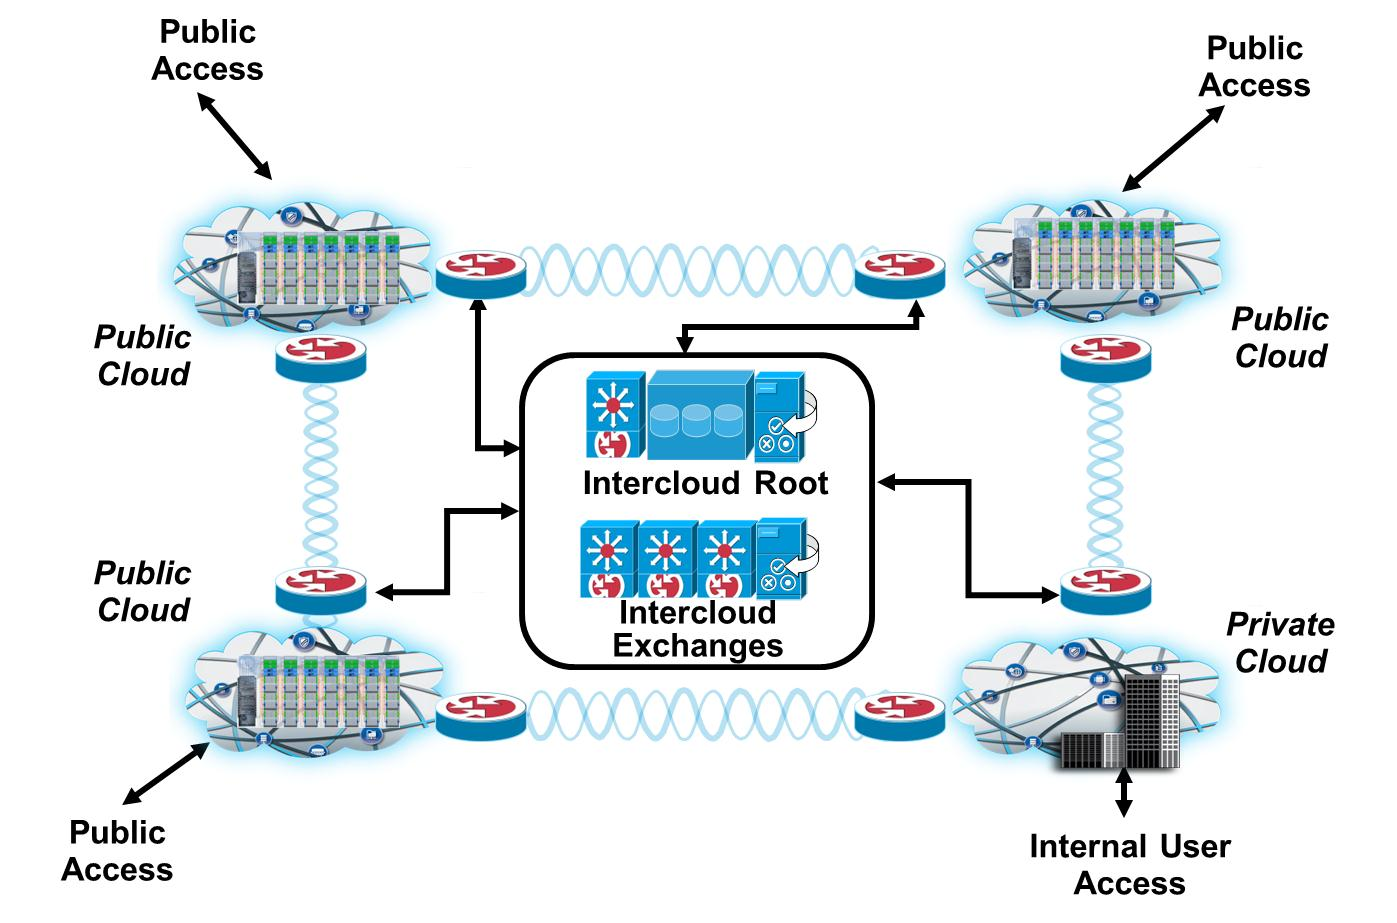
\includegraphics[width=0.78\textwidth]{img/testbed-technology.jpg}
  \caption{IEEE Intercloud Testbed Architecture}
  \label{fig:IEEE Intercloud Testbed Architecture}
\end{figure}

% paragraph IEEE Intercloud - (end)


\paragraph{\textbf{pkgcloud}} % (fold)
\label{par:pkgcloud }

is an open source standard library that abstracts differences between several cloud providers, by offering a unified vocabulary for services like storage, compute, DNS, load balancers, so the application developer does not have to be concerned with creating different implementations for each cloud. Instead, just make the provision in the one that is most cost-effective. Currently, it only supports applications built using Node.js.


% paragraph paragraph_name (end)

\paragraph{\textbf{Eucalyptus}} % (fold)
\label{par:Eucalyptus}

is a free and open source software to build Amazon Web Services Cloud like architectures for a private and/or hybrid Clouds. From the three solutions described, Eucalyptus is the one that is more deeply entangled with the concept of a normal Cloud, packing a: Client-side API, a Cloud Controller, S3 storage compliant modules, a cluster controller and a node controller, as seen in Figure~\ref{fig:eucalyptus}. Eucalyptus has all the components to build an entire cloud, however, since its compatible, specially, with Amazon Cloud, we can use Eucalyptus to migrate our services, or provision Amazon services, and work without having to deal with the application or the system itself.

\begin{figure}[h!]
  \centering
  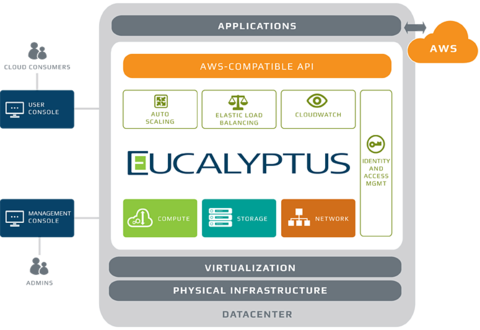
\includegraphics[width=0.95\textwidth]{img/eucalyptus-architecture.png}
  \caption{Eucalyptus Architecture}
  \label{fig:eucalyptus}
\end{figure}

This hybrid model provides a desired environment for a development, test and deploy stack, that can support Amazon Cloud with the elasticity necessary to sustain service during spikes. This way, a company that has its private cloud does not need to over provision in advance.

% paragraph Eucalyptus - (end)


% 
%---------{Volunteered resource sharing}--------------------------
% 
\subsection{Volunteered resource sharing}

Volunteered resource sharing networks enable the cooperation between individuals to solve higher degree computational problems, by sharing idle resources that otherwise would be wasted. These individuals may or may not have a direct interest with the problem that someone is trying to solve, however they share the resources for a common good. 

The type of computations performed in this Application-level networks (ALN), are possible thanks to the definition of the problem in meta-heuristics, describing it with as laws of nature\cite{Duda2013}, such as: Evolutionary algorithms (EA); Simulated annealing (SA); Colony optimization (ACO); Particle swarm optimization (PSO), Artificial Bee Colonies (ABC) and more. This process creates small individual sets of units of computation, known as `bag of tasks', easy to distribute through several machines in and executed in parallel.
                  
% Models for distributed computation:
% Global parallelization model - One population sharded in small sets computed by several slaves
% Island Model - The population is divided in subpopulation that can run in heterogeneous machines (this is the most common in distributed computing)
% Master-Salve Model - One central pop that communicates and collects data from others              





\subsubsection{3.2.1 Hybrid and Community Clouds}

A community cloud is a network of large scale, self-organized and essentially decentralized computing and storage resources. The main focus is on free economic and censorship wise, putting the user back in control of the information, giving them freedom to share content without censorship or a company interest. The term `User Centric Cloud' appears on \cite{Barraca2011}, where the resources are made available by individuals, but with a common API, similar to a centralized Cloud, where users that participate in the effort can also use others resources.

One major trend in Community Cloud computing is not only to share and trade computing resources, but also to build the actual physical network in which they are shared, this is known as Community Networks or ``bottom-up networking''. Community Networks such as guifi.net and Athens Wireless Metropolitan Network (AWMN) have together more than 22500 nodes providing localized free access to content, without the need to contract from an Internet provider.

CONFINE\cite{Navarro} is an European effort that has the goal to federate existing community networks, creating an experimental testbed for research on community owned local IP networks. From this project, resulted Community-Lab,\footnote{http://community-lab.org/ - seen on December 2013} a federation between guifi.net, AWMN and FunkFeuer (community network from Vienna and Graz, Austria), with the goal of carrying out experimentally-driven research on community-owned open networks.


% ``Scalable, self-organized and decentralized IP networks and services built and operated by citizens for citizens'' Navarro

\subsubsection{3.2.2 Cycle and Storage Sharing, using Volunteer Resource Systems}

When we talk about peer-to-peer applications, most people will remember volunteered storage sharing, as it most widely known for its ability to distribute content, thanks to the illegal distribution of copyrighted software and media. However if we take a look at the whole spectrum of volunteer resource systems, we will see that are two categories, one for content sharing and the second one for cycle sharing, the second is known today as Public Computing.

Storage and content sharing systems are the popular type from the two categories of peer-to-peer systems, specially because their ability to distribute content without legal control, which after their success, systems like Napster\footnote{http://napster.com - seen on December 2013} were legally forced to shutdown. One of the key benefits of using a peer-to-peer storage sharing system is their ability to optimize the usage of each individual user limited bandwidth, enabling file partitioned transfers from multiple users, using the hash of each partition or chunk to prove its integrity. Each file availability grows organically with the interested in that file, because more copies will exist in the network. Other examples of this type of system are: KaZaA\footnote{http://www.kazaa.com/}, BitTorrent\footnote{http://www.bittorrent.com/} and Freenet\cite{Clarke2001}.

The second category is that of systems that fit into the domain of Public Computing, where users share their idle computer cycles; this can be done by starting or resuming a computing process when the user is not performing any task that is relevant for him/her, or by establishing the tasks as low priority processes, so it does not affect the user experience. One way of doing this is using a screen saver, so the shift to an idle state is obvious to the machine. These systems are possible because we can divide bigger computational jobs into smaller tasks that can run independently and in parallel, again this is known as the ``bag-of-tasks'' model of distributed computing. Several systems using this currently are Folding@Home, Genome@Home\cite{Larson2002} and SETI@Home\cite{Anderson2002}\cite{Korpela2001}, all BOINC\cite{Anderson2015} based. However these systems work in a one way direction: volunteers to the network do not have the possibility to use the network for its own use; nuBOINC\cite{Silva2008}, enables contributers to take advantage of the network by adding extensions to the platform that enable every user to submit jobs, adding more flexibility towards the goal in which the shared computer cycles are used. 

Another interesting research on this field is moving the logic necessary for processing some data, alongside the data, this is known as Gridlet\cite{Costa2012}\cite{Rodrigues}, a unit of workload. This approach enables a more dynamic use of volunteer resource systems with the possibility of: having different goals for the same Grid, optimize the resources available of one machine by gathering different type of tasks in one machine, reduce the cost to start using a Grid for distributed computation.

\subsubsection{3.2.3 Peer-to-Peer Networks and Architectures -}  
Efficient resource discovery mechanisms are fundamental for a distributed system success, such as grid computing, cycle sharing or web application's infrastructures\cite{Ranjan2006}, although in the centralized model, by keeping data bounded inside a data center, we have a stable and scalable way for resource discovery, this does not happen in a P2P network, where peers churn rate can vary greatly, there is no way to start new machines on demand for high periods of activity, the machines present are heterogeneous and so is their Internet connectivity, creating an unstable and unreliable environment. To overcome these challenges, several researches have been made to optimize how data is organized across all the nodes, improving the performance, stability and the availability of resources. The following paragraphs will describe the current state of the art P2P organizations, typically categorized in P2P literature as Unstructured or Structured\cite{Milojicic2003}, illustrated in Figure~\ref{fig:Different types of P2P Overlay networks organizations}.

\begin{figure}[bh!]
  \begin{center}
    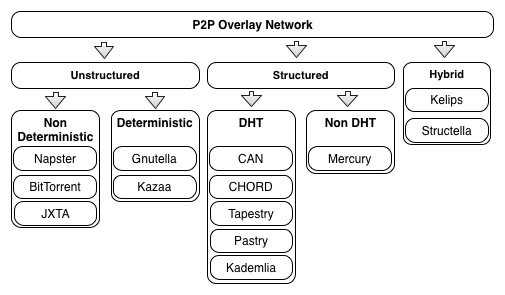
\includegraphics[width=0.75\textwidth]{./img/p2porganizations.jpg}
  \end{center}
  \caption{Different types of P2P Overlay networks organizations}
  \label{fig:Different types of P2P Overlay networks organizations}
\end{figure}


\paragraph{\textbf{Unstructured -}} % (fold)
\label{par:Unstructured}

We call `Unstructured' to a P2P system that doesn't require or define any constraint for the placement of data, these include Napster, Kazaa and Gnutella, famous for its file sharing capabilities, where nodes can share their local files directly, without storing the file in any specific Node. There is however a `caveat' in the Unstructured networks, by not having an inherent way of indexing the data present in the network, performing a lookup results of the cost of asking several nodes the whereabouts of a specific file or chunk of the file, creating a huge performance impact with an increasing number of nodes. 

In order to calibrate the performance, Unstructured P2P networks offer several degrees of decentralization, one example is the evolution from Gnutella 0.4\cite{Definition2003} to Gnutella 0.6 \cite{T.Klingberg2002}\cite{Ripeanu2002a}, which added the concept of super nodes, entities responsible for storing the lookup tables for the files in parts of the network they are responsible for, increasing the performance, but adding centralized, single points of failure. 

Unstructured networks are classified\cite{Ranjan2006} in two types: deterministic and non-deterministic, defining that in a deterministic system, we can calculate before hand the number of hops needed to perform a lookup, knowing the predefined bounds, this includes systems such as Napster and BitTorrent\cite{Cohen2009}, in which the file transfers are decentralized, the object lookup remains centralized, keeping the data for the lookup tables stored in one place, which can be gathered by one of two ways: (i) peers inform directly the index server the files they have; or (ii) the index server performs a crawling in the network, just like a common web search engine, this gives this network a complexity of O(1) to perform a search, however systems like Gnutella 0.6, which added the super node concept, remain non deterministic because it's required to execute a query flood across all the super nodes to perform the search.

% paragraph Unstructured and Non-Deterministic (end)

\paragraph{\textbf{Structured with Distributed Hash Tables -}} % (fold)
\label{par:Structured with Distributed Hash Tables}

Structured P2P networks have an implicit way of allocating nodes for files and replicas storage, without the need of having any specie of centralized system for indexing, this is done by taking the properties of a cryptographic hash function \cite{Bakhtiari}\cite{Kargerl}\cite{Preneel1999}, such as SHA-1\cite{D.Eastlake3rdMotorola;P.JonesSystems2001}, which applies a transformation to any set of data with a uniform distribution of possibilities, creating an index with O(log(n)) peers, where the hash of the file represents the key and gives a reference to the position of the file in the network.

DHT's such as Chord\cite{Stoica2001}, Pastry\cite{Rowstron2001} and Tapestry\cite{Zhao2001}, use a similar strategy, mapping the nodes present in the network inside an hash ring, where each node becomes responsible for a segment of the hash ring, leveraging the responsibility to forward messages across the ring to its `fingers'(nodes that it knows the whereabouts). Kademlia\cite{Maymounkov} organizes its nodes in a balanced binary tree, using XOR as a metric to perform the searches, while CAN\cite{Handley} introduced and a several dimension indexing system, in which a new node joining the network, will split the space with another node that has the most to leverage.

Evaluating the DHT Structured P2P networks raises identifiable issues, that result as the trade-off of not having an centralized infrastructure, responsible for railing new nodes or storing the meta-data, these are: (i) generation of unique node-ids is not easy achievable, we need always to verify that the node-id generated does not exist, in order to avoid collisions; (ii) the routing table is partitioned across the nodes, increasing the lookup time as it scales.

Table \ref{table:Complexity of structured P2P systems using a DHT}, showcases a comparison of the studied DHT algorithms.

\begin{table}
  \centering
  \begin{tabular}{| p{1.3cm} | p{2.0cm} | p{2.9cm} | p{3.2cm} | p{1.6cm} | p{1.8cm} | p{1.8cm} |}
    \hline                        
    \textbf{P2P system} & \textbf{Overlay Structure} & \textbf{Lookup Protocol} & \textbf{Networking parameter} & \textbf{Routing table size} & \textbf{Routing complexity} & \textbf{Join/leave overhead} \\
    
    \hline
    Chord & 1 dimension, Hash ring & Matching key and NodeID & n= number of nodes in the network & O(log(n)) & O(log(n)) & O(log(n)\textsuperscript{2}) \\
    
    \hline
    Pastry & Plaxton style mesh structure & Matching key and prefix in NodeID & n= number of nodes in the network, b=base of identifier & O(log\textsubscript{b} (n)) & O(b log \textsubscript{b}(n)+b) & O(log(n)) \\
    
    \hline
    CAN & d-dimensional ID Space & Key value pair map to a point P in the D-dimensional space & n= number of nodes in the network, d=number of dimensions & O(2d) & O(d n\textsuperscript{1/2}) & O(2d) \\
    
    \hline
    Tapestry & Plaxton style mesh structure & Matching suffix in NodeID & n=number of nodes in the network, b=base of the identifier & O(log\textsubscript{b}(n)) & O(b log \textsubscript{b} (n)+b) & O(log(n)) \\
    
    \hline  
    Kademlia & Binary tree & XOR metric & n=number of nodes, m=number of different bits (prefix) & O(log(n)) & O(log\textsubscript{2}(n)) & not stable \\
    \hline      
  \end{tabular}
  \caption{Summary of complexity of structured P2P systems}
  \label{table:Complexity of structured P2P systems using a DHT}
\end{table}

% paragraph Structured with Distributed Hash Tables (end)

\paragraph{\textbf{Structured without Distributed Hash Tables -}} % (fold)
\label{par:Structured without Non-Distributed Hash Tables}

Mercury\cite{Bharambe}, a structured P2P network that uses a non DHT model, was designed to enable range queries over several attributes that data can be dimensioned on, which is desired on searches over keywords in several documents of text. Mercury design offers an explicit load balancing without the use of cryptographic hash functions, organizing the data in a circular way, named `attribute hubs'.

% paragraph Structured without Non-Distributed Hash Tables (end)

% \paragraph{\textbf{Hybrid -}} % (fold)
% \label{par:Hybrid}

% %TODO Structella , Kelips

% NOTE: Not sure if should include this, doesn't really include anything that new

% In recent developments, new generation P2P systems have evolved to combine both unstructured and structured P2P networks. We refer to this class of systems as hybrid. Structella [27] is one such P2P system that replaces the random graph model of an unstructured overlay (Gnutella) with a structured overlay, while still adopting the search and content placement mechanism of unstructured overlays to support complex queries. Other hybrid P2P design includes Kelips [60] and its variants. Nodes in Kelips overlay periodically gossip to discover new members of the network, and during this process nodes may also learn about other nodes as a result of lookup
% 12
% communication. Other variant of Kelips [56] allows routing table entries to store information for every other node in the system. However, this approach is based on assumption that system experiences low churn rate [70]. Gossiping and one-hop routing approach has been used for maintaining the routing overlay in the work [108]. In Table 4, we summarize the different P2P routing substrate that are utilized by the existing algorithms for organizing a GRIS.


% paragraph Hybrid (end)

\subsubsection{3.2.4 Fault Tolerance, Load Balancing, Assurance and Trust -}

Volunteer resource sharing means that we no longer have our computational infrastructure confined in a well monitored place, introducing new challenges that we have to address \cite{Koloniari2005} to maintain the system running with the minimum service quality. These issues can be: scalability, fault tolerance, persistence, availability and security\cite{Wallach} of the data and that the system doesn't get compromised. This part of the document serves to describe the techniques implemented in previous non centralized systems to address this issues.

\paragraph{\textbf{Fault Tolerance, Persistence and Availability}} % (fold)
\label{par:Fault Tolerance, Persistence and Availability}

are one of the key challenges in P2P community networks, due to it's churn uncertainty, making the system unable to assume the availability of Node storing a certain group of files. Previous P2P systems offer a Fault Tolerance and Persistence by creating file replicas, across several Nodes in the network, one example is PAST\cite{Rowstron2001}\cite{Rowstron2001a}, a system that uses PASTRY routing algorithm, to determine which nodes are responsible to store a certain file, creating several different hashes which corresponds to different Nodes, guaranteeing an even distribution of files across all the nodes in the network. DynamoDB\cite{Decandia2007}, a database created by Amazon to provided an scalable NOSQL solution, uses a storage algorithm, inspired by the Chord routing algorithm, in which stores file replicas in the consequent Nodes, in order to guarantee easy lookup if one of the Nodes goes down.

The strategy presented by the authors of PAST to provide high availability, is an intelligent Node system, that use a probabilistic model, able to verify if there is an high request for a file, deciding to keep a copy and avoiding to overload the standard Node with every request that is made.

% paragraph Fault Tolerance, Persistence and Availability (end)

\paragraph{\textbf{Load Balancing}} % (fold)
\label{par:load_balancing}

in an optimal state, can be defined as having each node sharing roughly 1/N of the total load inside the network, if a Node has a significantly hight load compared with the optimal distribution, we call it a `heavy' node. There has been some research to find a optimal way to balance the load inside a P2P network, namely:

\begin{itemize}
   \item Power of Two Choices\cite{Byers} - Uses multiple hash functions to calculate different locations for an object, opts to store it in the least loaded node, where the other Nodes store a pointer. This approach is very simple, however it adds a lot of overhead when inserting data, however there is a proposed alternative of not using the pointers, which has the trade-off of increasing the message overhead at search.
   \item Virtual Servers\cite{Rao2003} - Presents the concept of virtualizing the Node entity to easy transfer it amongst the machines present in the P2P network. It uses two approaches, `one-to-one', where nodes contact other Nodes inside the network with the expectation of being able to trade some of the load, shifting a virtual server, or an `one-to-many/many-to-many' in which a directory of load per node is built, so that a node can make a query in order to find it's perfect match to distribute his load. Virtual Servers approach has the major issue of adding a extra amount of work to maintain the finger tables in each node.
   \item Thermal-Dissipation-based Approach\cite{Rieche} - Inspired by the heat expansion process, this algorithm shifts nodes position inside the hash ring windows of load responsibility, in a way that the load will implicitly flow from a node to it's close peers.
   \item Simple Address-Space and Item Balancing\cite{Karger2004} - It is an iteration over the virtual servers, by assigning several virtual nodes to each physical node, where only one of which is active at a time and this is only changed if having a different nodeId distribution in the network brings a more load balanced hash ring
 \end{itemize} 

S. Rieche, H. Niedermayer, S. Götz and  K. Wehrle from the University of Tübingen, made a study comparing this different approaches in a scenario using the CHORD routing algorithm, using a SHA-1 as the hashing function, with 4096 nodes and 100.000 to 1.000.000 documents and executing up to 25 runs per test, the results can be observed in the Figure ~\ref{fig:lbcomp}


\begin{figure}[h!]
  \centering
  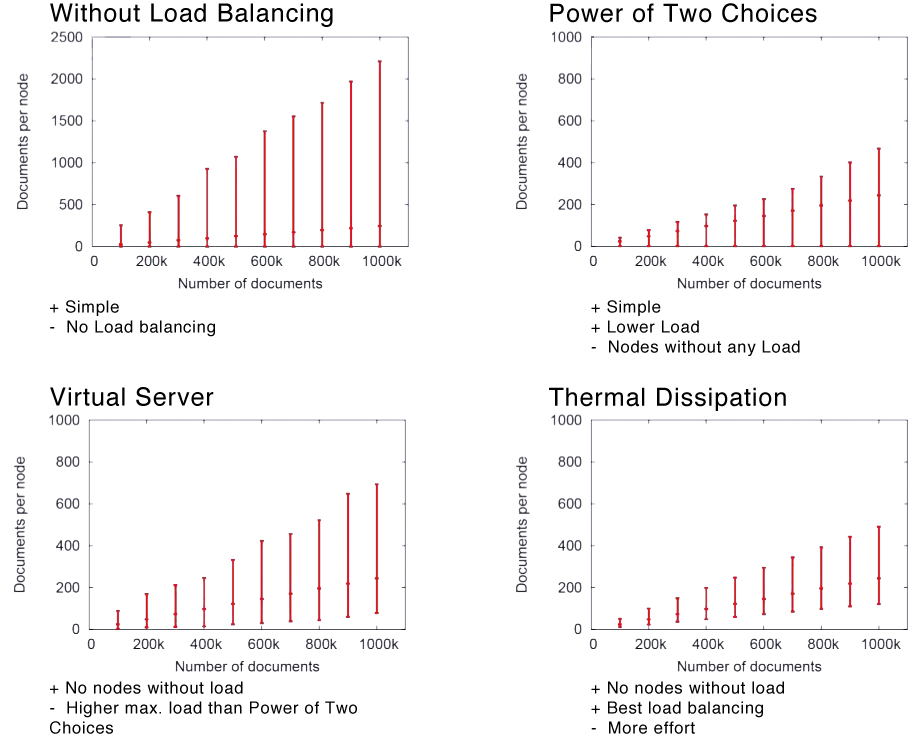
\includegraphics[width=1\textwidth]{img/lb.jpg}
  \caption{Load balancing approaches comparison}
  \label{fig:lbcomp}
\end{figure}


% paragraph load_balancing (end)

\paragraph{\textbf{Assurance and Trust}} % (fold)
\label{par:Assurance and Trust}

in a P2P network is an interesting challenge due to the lack of control over the machines that are willing to share with their resources, in order to achieve it, several strategies have been developed to maintain the integrity of the data using Cryptography, Reputation modeling schemes based on it's node previous record and also economic models, that resemble our own economy, but to share and trade computational resources.

Starting with the Cryptographic techniques, storage systems such as PAST give the option to the user to store encrypted content, disabling any other user, that does not have the encryption key, to have access to the content itself, this is a technique that comes from the Client-Server model, adapted to P2P environment, however, other cryptography technique benefits such as user authorization and identity, cannot be directly replicated into a P2P network without having a centralized authority to issue this validations, one of the alternatives is using distributed signature strategy, known as Threshold Cryptography \cite{Desmedt;1998}, where an access is granted if validated if several peers (a threshold), validates it's access, one implementation of Threshold Cryptography can be see in a P2P social network\cite{Afify} in order to guarantee privacy over the contents inside the network. 

Trust in a P2P system, as mentioned, is fundamental to it's well behaved functioning, not only in terms of data privacy, but also in giving the deserved resources to the executions that mostly need them, avoiding misbehaved peer intentions that can be a result of an Attack to jeopardize the network, one example is the known Sybil attack\cite{Douceura}. To achieve a fair trust sharing system, several metrics for a reputation mechanism have been developed \cite{Marti}, these can be seen in Table \ref{table:reputation}.

\begin{table}
  \centering
  \begin{tabular}{| c | c | c |}
    \hline                        
    \multicolumn{3}{|c|}{Reputation Systems} \\

    \hline                        
    Information Gathering & Scoring and Ranking & Response \\
    
    \hline                        
    Identity Scheme & Good vs. Bad Behavior & Incentives \\
    Info. Sources & Quantity vs. Quality & Punishment \\
    Info. Aggregation & Time-dependence &   \\ 
    Stranger Policy & Selection Threshold &   \\ 
      & Peer Selection &   \\ 

    \hline                           
  \end{tabular}
  \caption{Reputation system components and metric}
  \label{table:reputation}
\end{table}

Incentives for sharing resources\cite{Golle2001} can in the form of money rewards, greater speed access(used in Napster and some bittorrent networks) or it can be converted to a interchangeable rate to trade for more access to resources, giving the birth of economic models\cite{Filipe2011}\cite{Vishnumurthy}, that model the traded resources as a currency in which a peer has to trade in order to use the network.

% Economic Models
% * Gridlet Economics: Resource Management Models and Policies for Cycle-Sharing Systems
% * KARMA : A Secure Economic Framework for Peer-to-Peer Resource Sharing  (note: stores reputation remotly) Nead to Read


% paragraph Assurance and Trust (end)

% 
%---------{Resource sharing using the Web as platform}------------
% 
\subsection{Resource sharing using the Web platform} 

One of the main focuses with the proposed work, is to take advantage of the more recent developments of the Web platform to make the intended design viable (presented in section 4), the system depends on very lower level components such as:
\begin{itemize}
  \item High dynamic runtime for ongoing updates to the platform and specific assets for job execution
  \item Close-to-native performance for highly CPU-bound jobs
  \item Peer-to-peer interconnectivity
  \item Scalable storage and fast indexing
\end{itemize}

Therefore, we present in this section the relevant components present or undergoing a development process for the Web platform, such as: Javascript, Emscripten, IndexedDB, WebRTC and HTTP2.0. These will coexist as key enablers for  the necessary features to such a distributed shared resource system:

\subsubsection{3.3.1 Web Platform}

Since the introduction of AJAX\cite{Google/Mozzila/Opera}, the web has evolved into a new paradigm where it left being a place of static pages, known as Web 1.0. Nowadays, we can have rich web applications with degrees of interaction and levels of performance close to a native application. The programming languages that power the Web Platform, in special HTML, CSS and JavaScript\cite{Ecma2009}, have been subject to several changes, enabling `realtime' data transfers and fluid navigations through content. Javascript, an interpreted language with an high dynamic runtime, has proven to be the right candidate for a modular Web Platform, enabling applications to evolve continuously over time, by simply changing the pieces that were updated.

\textbf{Emscripten}\cite{Zakai2011}, a LLVM(Low Level Virtual Machine) to JavaScript compiler, enabled native performance on Web apps by compiling any language that can be converted to LLVM bytecode, for example C/C++, into JavaScript. This tool enabled native game speed on the browser, where two of the major examples are the project Codename: ``BananaBread''\footnote{Mozilla, BananaBread,  URL: https://developer.mozilla.org/en/demos/detail/bananabread, seen in December 2013} and ``Epic Citadel''\footnote{Mozilla, Epic Citadel,  URL: http://www.unrealengine.com/html5/, seen in December 2013}, in which Mozilla used Ecmascripten to port the entire Unreal Engine 3 to JavaScript. In Figure~\ref{fig:dan}, we can see a comparison of the performance of several algorithms, running on Dalvik, Android Java runtime, asm.js, the subset of Javascript that the code in C/C++ is transformed into when compiled with Emscripten and Native, the same C/C++ but running on a native environment. The results are very interesting, specially in the first test, where asm.js outperforms native. The explanation for this is due to the fact that BinaryTrees use a significant amount of `malloc' invocations, which is an expensive system call, where in asm.js, the code uses typed arrays, using `machine memory', which is flat allocated in the beginning of the execution for the entire run.

\begin{figure}[h!]
  \centering
  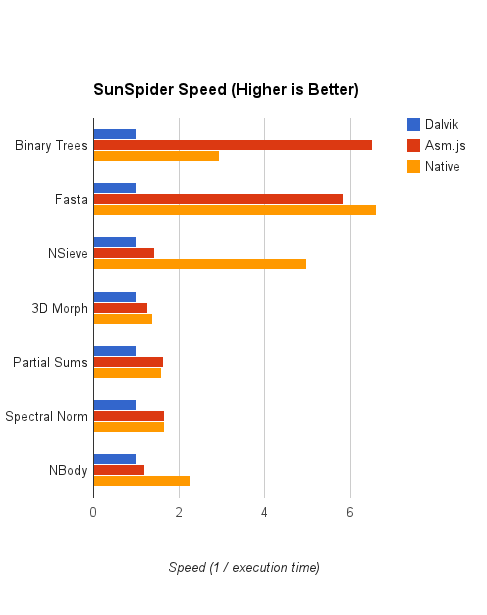
\includegraphics[width=0.7\textwidth]{img/Dalvik-vs-ASM-vs-Native-edited}
  \caption{Dalvik vs. ASM.js vs. Native performance}
  \label{fig:dan}
\end{figure}

\textbf{WebRTC}\cite{IanHickson2013}, a technology being developed by Google, Mozilla and Opera, with the goal of enabling Real-Time Communications in the browser via a JavaScript API. WebRTC brings to the browser the possibility of peer-to-peer interoperability. Peers perform their handshake through a `Signaling Server'. The signaling server will exchange the `ICE(Interactive Connectivity Establishment) candidates' of each peer as this serves as an invite so a data-channel can be opened, a visualization of this process can be seen in Figure~\ref{fig:webrtc}. Since most of the browsers sit behind NAT, there is another server, named `Turn'(Relay), which tells to each browser their public IP in the network. WebRTC, although being built with the goal of real-time voice and video communications, has also been shown as a viable technology do distribute content, as seen in PeerCDN and SwarmCDN\cite{Vogt}.

\begin{figure}[h!]
  \centering
  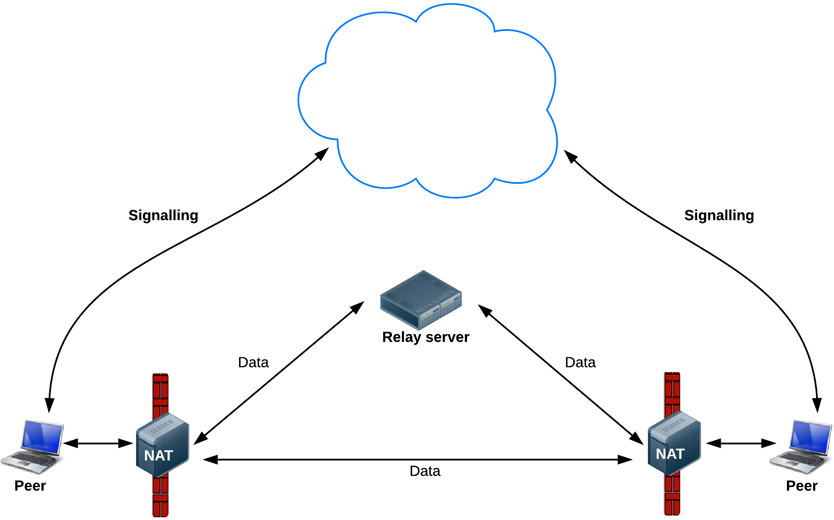
\includegraphics[width=0.7\textwidth]{img/webrtc.png}
  \caption{Example of a WebRTC session initiation}
  \label{fig:webrtc}
\end{figure}

% 
% There is also Jingle
% https://github.com/legastero/jingle.js
% Jingle is an extension of XMPP that enables P2P and communication over RTC
% 


\textbf{`level.js'} offers an efficient way to store larger amounts of data in the browser machine persistent storage, its implementation works as an abstraction on top of the leveldown API on top of IndexedDB\cite{Recommendation2013}, which in turn is implemented on top of the LevelDB\cite{JeffreyDean;SanjayGhemawat}, an open source on-disk key-value store inspired by Google BigTable. IndexedDB is an API for client-side storage of significant amounts of structured data and for high performance searches on this data using indexes. Since `level.js' runs on the browser, we have an efficient way to storage data and quickly retrieve it.

One of the latest improvements being built for the Web Platform is the new HTTP spec, \textbf{HTTP2.0}\cite{Thomson2013}, this next standard after HTTP1.1 which aims to improve performance towards a more realtime oriented web, while being retrocompatible at the same time. Several advancements in this new spec are:

\begin{itemize}
  \item Parallel requests - HTTP1.1 was limited by a max of 6 parallel requests per origin and taking into account that the mean number of assets is around one hundred when loading an webapp, it means that transfers get queued and slowed down. In order to overcome this, we could distribute the assets through several origins in order to increase the throughput. However this optimization backfired when in mobile, since there was a lot of signaling traffic in TCP layer, starving the user connection. HTTP2.0 no longer has this constraint.
  \item Diff updates - One of the web developer favorites has been concatenating their javascript files so the response payload decreases, however, in modern webapps, most of the time, we do not want the user to download the entire webapp again, but only some lines of code referring to the latest update. With diff updates, the browser will only receive what has been changed.
  \item Prioritization and flow control - Different webapp assets have different weights in terms of user experience, with HTTP2.0, the developer can set priorities so the assets arrive by order.  A simple flow control example can be seen on Figure~\ref{fig:http2dataflow}, where the headers of the file gain priority as soon as they are ready, and get transfered immediately. 
  \item Binary framing - In HTTP2.0, binary framing is introduced with the goal of creating more performant HTTP parsers and encapsulating different frames as seen on Figure~\ref{fig:binaryframing}, so they can be send in an independent way.
  \item HTTP headers compression - HTTP2.0 introduces an optimization with headers compression\cite{Ruellan2013} that can go to a minimum of 8 bytes in identical requests, against the 800 bytes in HTTP1.1. This is possible because of the state of the connection is maintained, so if a identical requests is made, changing just one of the resources (for example path:/user/a to path:/user/b), the client only has to send that change in the request.
  \item Retrocompatibility - HTTP2.0 respects the common headers defined by HTTP1.1, it doesn't include any change in the semantics.
\end{itemize}

\begin{figure}[htbp]
  \centering
  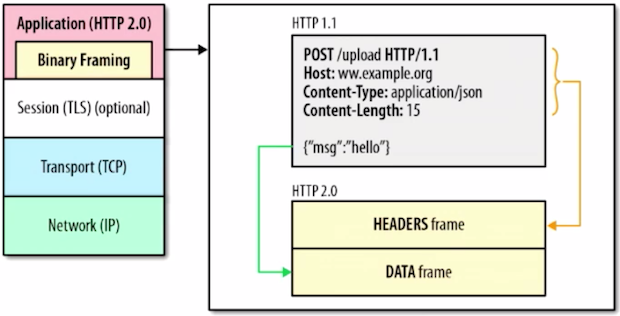
\includegraphics[width=0.75\textwidth]{img/http2binaryframing.png}
  \caption{HTTP2.0 Binary framing}
  \label{fig:binaryframing}
\end{figure}

\begin{figure}[htbp]
  \centering
  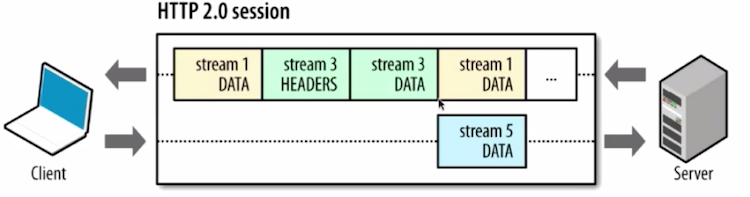
\includegraphics[width=0.75\textwidth]{img/http2dataflow.png}
  \caption{Example of an HTTP2.0 dataflow}
  \label{fig:http2dataflow}
\end{figure}


\subsubsection{3.3.2 Previous attempts on cycle sharing through web platform}
The first research of browser-based distributed cycle sharing was performed by Juan-J. Merelo, et. al., which introduced a Distributed Computation on Ruby on Rails framework\cite{Merelo2007}. The system used a client-server architecture in which clients, using a browser would connect to a endpoint, where they would download the jobs to be executed and sent back the results. In order to increase the performance of this system, a new system\cite{Duda2013} of browser-based distributed cycle sharing was creating using Node.js as a backend for very intensive Input/Output operations\cite{Tilkov2010}, with the goal of increased efficiency, this new system uses normal webpages (blogs, news sites, social networks) to host the client code that will connect with the backend in order to retrieve and execute the jobs, while the user is using the webpage, this concept is known as parasitic computing\cite{Barabasi2001}, where the user gets to contribute with his resources without having to know exactly how, however since it is Javascript code running on the client, any user has access to what is being processed and evaluate if it presents any risk to the machine.


\textbf{Analysis and discussion}

The related work presented was researched with the goal of deepen the knowledge about current strategies for resource sharing, as we intend to present a new one using the Web Platform. The concept of Gridlet, akin to those seen as well in state of the art databases such as Joyent's Manta,\footnote{http://www.joyent.com/products/manta - seen in December 2013} which bring the computation to/with the data, reducing the possibility of a network bottleneck and increases the flexibility to use the platform for new type of jobs, will very important. To enable this new Cloud platform on using browsers, it is important to understand how to elastically scale storage and job execution, as in \cite{Silva2011}, but in peer-to-peer networks: therefore a study of the current algorithms and its capabilities was needed. Lastly, browsing the web is almost as old as the Internet itself, however on the last few years, we are seeing the Web Platform rapidly changing, and enabling new possibilities with peer-to-peer technology e.g. WebRTC; otherwise, it would not be possible to create browserCloud.js.

%!TEX root = ../index.tex

% 
% Architecture
% 

\section{Analysis and discussion of the architecture}

In this section we describe our proposed architecture for the remaining implementation work. The software stack is composed by several subsystems that have one specific goal, exposing a well known API, this way the subsystems become interchangeable. These subsystems include:

\begin{itemize}
  \item \textbf{Communication service} - Responsible for routing messages between nodes in the DHT.
  \item \textbf{Service router} - Processes the messages that have as destiny the its node, the goal is to call the right service (storage, reputation mechanism, job execution, etc) accordingly. One other key aspect is the ability to attach new services during the runtime.
  \item \textbf{Storage service} - Stores any data that requires persistence in the network, such as job logs, reputation logs and file meta data and chunks.
  \item \textbf{Job coordination} - A subsystem responsible for coordinating jobs requested by the client, keeping state and assuring its completion/
  \item \textbf{Job execution} - Execution of jobs, gathering all the necessary assets (image processors, sound wave manipulators, etc) to complete the job/
  \item \textbf{Reputation Mechanism} - Validate user behavior and right to take different responsibilities in the network.
  \item \textbf{Client API and CLI} - In order to interact with the network, we offer an API and a CLI with Unix type instructions and familiar web cloud instructions that developers are familiar.
  \item \textbf{Rendezvous points} - The only centralized component in this architecture, its purpose is for the clients to have a way to connect to the overlay network. 
\end{itemize}

We can observe how this subsystems interconnect with each other by observing Figure~\ref{fig:softwarestack}

\begin{figure}[h!]
  \centering
  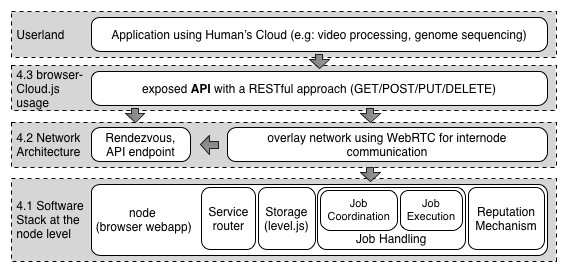
\includegraphics[width=0.9\textwidth]{img/softwarestack.jpg}
  \caption{browserCloud.js Software Stack}
  \label{fig:softwarestack}
\end{figure}


\subsection{Network Architecture}

Network architecture can be seen on Figure \ref{fig:overallarchitecture}). Nodes (volunteer computers), are divided into two Chord DHTs with the purpose of separating the nodes with storage responsibility from the ones with only computing responsibility. The reason behind this decision is due to the high churn rate in a P2P network. Keeping the files in nodes have proven to be more trustworthy for staying longer in the network makes the system more robust by keeping the file replica level stable. This also reduces the message overhead that would require to keep the replica level in a more inconsistent environment. Nevertheless, the more volatile nodes are perfect for short computing operations, till they proven to be trustworthy to `ascend' in the network.

\begin{figure}[h!]
  \centering
  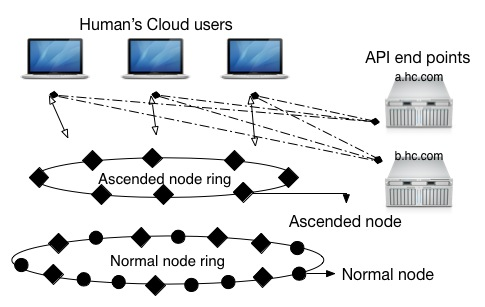
\includegraphics[width=0.8\textwidth]{img/overall.jpg}
  \caption{browserCloud.js network architecture}
  \label{fig:overallarchitecture}
\end{figure}

Since browsers cannot effectively have a static IP nor have a DNS record updated on demand pointing to themselves, we designed the API endpoints as the rendezvous between browsers and clients.

\subsection{Software architecture at the node level}

At the node level, we divide the application into two fundamental services and three pluggable components, with the possibility for expansion, thanks to Javascript dynamic runtime, we can find this structure in Figure~\ref{fig:hcnode}.

In the communication layer, we find the DHT logic implemented to effectively propagate messages. One of the main goals with component is to be modular, so we can switch between different DHT algorithm if necessary, without affecting the rest of the application functionality.

Next, we have the Service Routing layer, this service is responsible to guide the message to the right component, enabling the architecture to be more modular, plugging in more components as it is needed. For example, when a node ascends and needs the storage component to fulfill his responsibility.

Last, we have the components, individual modules that do one thing and one thing well. Currently, we present the Storage module, responsible for holding the data; the Job Scheduler, responsible to orchestrate jobs issued by the users; the assets needed to execute the jobs and finally; the job executor, the module that will execute the jobs in a separate process using webworkers.

% Doug McIlroy, then head of the Bell Labs CSRC and contributor to Unix pipes,[1] summarised Unix philosophy as follows:[2]
% This is the Unix philosophy: Write programs that do one thing and do it well. Write programs to work together. Write programs to handle text streams, because that is a universal interface.

\begin{figure}[h!]
  \centering
  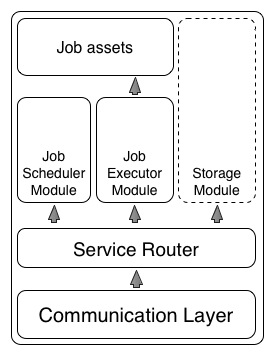
\includegraphics[width=0.35\textwidth]{img/node.jpg}
  \caption{browserCloud.js Node}
  \label{fig:hcnode}
\end{figure}

\subsection{Storage}

browserCloud.js storage happens in what it is named, the ``Ascended node ring'', these nodes have an higher reliability, making the storage system more stable, without the need of constantly burning computer cycles to maintain the files replica level.

Data stored in nodes can be:
\begin{itemize}
  \item File metadata (name of the file, size, location of the chunks, chunks hash);
  \item File chunks;
  \item Directories metadata - This way, bcls can be more efficient ;
  \item Job information (state, issuer, workflow);
  \item Reputation log;
\end{itemize}

We classify storage nodes into two types: 1) the `sKeeper', responsible for holding the metadata of the file and hashing each chunk to identify the `sHolder'; 2) `sHolder' nodes responsible to store the chunk into their system. This approach mitigates the possibility of having an highly unbalanced storage distribution, dividing each file in equal chunks across several nodes. As we can see in Figure~\ref{fig:chunking}, each chunk gets hashed more than one time with a different hash function, its purpose being to identify several Nodes that will be responsible to store a replica of the chunk. Also, in order to increase the fault tolerance of the system, we replicate the `sKeeper' responsibility in the two following nodes in the hashring, so if one of these fails, another is assigned.

\begin{figure}[h!]
  \centering
  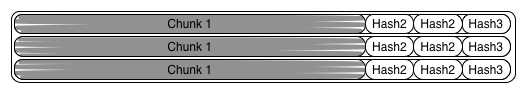
\includegraphics[width=0.7\textwidth]{img/chunking.jpg}
  \caption{A file partitioned in several chunks, each with its corresponding hashes that correspond to nodeIds}
  \label{fig:chunking}
\end{figure}

In Figure~\ref{fig:skeepersholder}, we can find the `sKeeper' and `sHolder' relationship. Only the sKeeper performs the chunk hashing and stores the information in the file lookup table. This happens one single time for each chunk, reducing several network hops per message on the consequent searches.

\begin{figure}[h!]
  \centering
  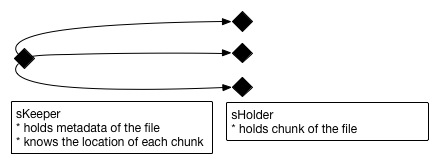
\includegraphics[width=0.7\textwidth]{img/skeepersholder.jpg}
  \caption{Representation of the Node responsible for the file(sKeeper) and it's individual chunk holders(sHolders)}
  \label{fig:skeepersholder}
\end{figure}

Each store file is chunked as soon as it enters the network, thus mitigating the risk that would be present if we were transferring files with considerable sizes all at once, starving the network and the node's heap. The only point where the file gets assembled together again is when it leaves the network and sent to the user, and even this could be made to perform chunk transfer in parallel to the client directly.

browserCloud.js adapts the Load Balancing virtual server's method, by using the same strategy of global load, but by transferring files between sHolders and not an entire virtual server, updating the respective sKeeper accordingly. Files are storage as objects in a indexedDB type storage, provided by the leveljs module. 

\subsection{Distributed Job Scheduling}

Job coordination is one of the main challenges in a completely distributed environment, in a sustainable and scalable way. Traditionally in the client-server model, we have the possibility to select one of the nodes to be the job coordinator. To implement this in a P2P network, we take advantage of the DHT, to select randomly one of the ascended nodes to be the `jKeeper', the node responsible for coordinating the job in an environment a P2P network.

The `jKeeper' is responsible for contacting the `sKeepers' of each individual file, and coordinate them to command each of `sHolder' to perform the desired computation on the file. All the steps during the computation are journaled in the Job log, stored with the coordinator, and replicated in the two following nodes for Fault Tolerance measure.

All the coordination takes place in the ascended Node ring, however, in order to take advantage of the normal node ring resources. `sHolders' are allowed to offload the computation to process this job in the `normal hash ring'. This is done by sending a probe, asking for `volunteers' for a job, when the threshold required is met, the orchestration starts, where the `sHolder' transfers the data and the assets necessary for processing it.

An example in pseudo-code can be analyzed below: \\

\textit{Client pseudo-code}
\begingroup
\scriptsize
\begin{verbatim}
var jobId = randomUniqueIdGenerator();
sendJob(jobId, job); // job object includes the files names being manipulated+assets
\end{verbatim}  
\endgroup



\textit{jKeeper pseudo-code}
\begingroup
\scriptsize
\begin{verbatim}
replicateJob(); // each job replica holder will ping the jKeeper to make sure progress 
// is made, if the node fails, other will assume its role
job.sKeepersList.forEach(function (sKeeper){
  commandJobExecution(job, sKeeper, statusReport);
  function statusReport(status){
    log(status);
  }  
}); //Job is complete
\end{verbatim}
\endgroup

\textit{sKeeper pseudo-code}
\begingroup
\scriptsize
\begin{verbatim}
var sHolders = this.getsHolders(job.filename);
sHolders.forEach(function(sHolder){
  commandTaskExecution(sHolder, taskReport);
  function taskReport(status){
    reportBack(status); // report to jKeeper
  }
});
\end{verbatim}
\endgroup

\textit{sHolder pseudo-code}
\begingroup
\scriptsize
\begin{verbatim}
if(smallTask && available) {
  doIt(task, taskReport);
} else {
  requestNormalNodesToExecute(task, taskReport)
}
function taskReport(status){
  reportBack(status); // report to sKeeper
}
\end{verbatim}
\endgroup



\subsection{Reputation Mechanism}

The reputation mechanism present will enable the network to identify the nodes that show more availability and have the necessary means to ascend and take a more important role. In order to evaluate each node, we define several metrics, these are: uptime, number of job completions, network throughput and computational resources (CPU) available, being the uptime, the most important, to assure stability. The reputation metric is calculated as follows: \\

$ \textbf{reputation} = \alpha * log(uptime) + \beta * log(job completions) + $ \\
$          \gamma * log(network throughput) + \delta * log (CPU)$

where: \\
  $\alpha+ \beta+ \gamma+ \delta = 1$; \\
  $\alpha > \beta + \gamma + \delta$;  \\

We chose to normalize the metrics and give more importance to the uptime of the system, because this is the one metric allowing a more stable network for storage.

The reputation of each node is stored with its node identifier on the `ascended hash ring'. Each time a job is completely successfully, this score gets updated and in case it reaches the required level to ascend, the jKeeper that was updating thus score will enable and deploy the remaining features (storage and job schedule module) it needed to join the ascended group. 

\subsection{Client API and CLI}

The client API goal is to be familiar to experienced developers using cloud providers today and at the same time, respect the Unix philosophy, where the job work flows are composed by a stream of assets, that do one thing and one thing well. It will support CRUD operations through a REST with JSON API, a filesystem-like interface (directories and objects), where user is identified by a username and it maps to the paths shown in Table~\ref{tbl:dirrepnet}: 

\begin{table}
  \begin{tabular}{ p{3cm} | p{9cm} }
  % \hline 
  Path & Description \\
  \hline 
  /:username/jobs/ & where new jobs can be inserted by the user \\
  \hline
  /:username/jobs-reports/ & Job status. The user is only able to read and delete the records, they are created by the system. \\
  \hline 
  /:username/home/ &  Private user store, only place where the user has write access \\
  \hline   
  /:username/reports/ & Usage and Access log reports. \\ 
  \hline   
  /nodes/ & Registry of all the nodes in the network with their metadata, the user can only read this folder. \\
  % \hline   
  \end{tabular}
  \caption{Directories representation inside the network}
  \label{tbl:dirrepnet}
\end{table}

We provide a REST API for the developer to use. The reason behind this design decision is to create a familiar interface to the majority of web developers. The server replying to these requests defined in Table~\ref{tbl:restapi}, can be a public or a private proxy, in the user machine, behind a company firewall or as a public service available to the community. Thus, it remains portable and does not lock in the user to a provider.

\begin{table}
  \begin{tabular}{ l | c | p{6cm} }
    \multicolumn{3}{ l }{\textbf{Directories}} \\
    Action: PutDirectory & \multicolumn{2}{l}{PUT /:username/home/[:directory]/:directory} \\
    Action: ListDirectory & \multicolumn{2}{l}{GET /:username/home/[:directory]/:directory} \\
    Action: DeleteDirectory & \multicolumn{2}{l}{DELETE /:username/home/[:directory]/:directory} \\
    \hline 
    \multicolumn{3}{ l }{\textbf{Files}} \\
    Action: PutFile & \multicolumn{2}{l}{PUT /:username/home/[:directory]/:filename} \\
    Action: GetFile & \multicolumn{2}{l}{GET /:username/home/[:directory]/:filename} \\
    Action: DeleteFile & \multicolumn{2}{l}{DELETE /:username/home/[:directory]/:filename} \\
    \multicolumn{3}{p{12cm}}{\textbf{note:} PutFile and GetFile, the body of the request and response  respectively is the file} \\
    \hline 
    \multicolumn{3}{ l }{\textbf{Jobs}} \\
    Action: CreateJob & \multicolumn{2}{l}{PUT /:username/jobs} \\
    Action: CancelJob & \multicolumn{2}{l}{DELETE /:username/jobs/:jobId} \\
    Action: ListJobs & \multicolumn{2}{l}{GET /:username/jobs} \\
    Action: GetJob & \multicolumn{2}{l}{GET /:username/home/jobs/:jobId} \\
    Action: GetJobOutput & \multicolumn{2}{l}{GET /:username/jobs-reports/:jobId} \\
    \hline \\
    \multicolumn{3}{p{12cm}}{\textbf{Note:} Create Job, several arguments are passed, most importantly, an array named ``phases'' that includes the orders with assets necessary in order to execute the job(e.g. `grep -ci' or if its a new asset, it should be a JS object with a closure.)} \\
    \hline 
  \end{tabular}
  \caption{browserCloud.js REST API Draft}
  \label{tbl:restapi}
\end{table}

We are also including a CLI\footnote{CLI - Command Line Interface} tool to enable quickly bash scripts for computation jobs and file storage, this CLI uses in the background the API defined in Table~\ref{tbl:restapi}. For example, if we are looking for video transcoding: ``hcjob create /path/to/file | ffmpeg | /path/to/out.webm''. The rest of the commands are:
  
\begin{itemize}
  \item \textbf{\$ bcls}  - List files in a directory
  \item \textbf{\$ bcget} - Get an object stored
  \item \textbf{\$ bcput} - Store an object
  \item \textbf{\$ bcjob} - Initialize a job   
\end{itemize} 

%!TEX root = ../index.tex

% 
% Evaluation
% 

\section{Evaluation}

The proposed system will be evaluated with the goal of comparing to existing centralized non P2P cloud, P2P distributed job computing and storage. The desired output of this analysis will be to produce a quantifiable and comparable metrics to other systems, taking into account its scalability, resilience, availability, processing power and latency. In the end, we expect to have an ``type of application/solution'', mentioning the advantages present using browserCloud.js in comparison with the other systems, such as table~\ref{tbl:cloudcomparisson}.


\subsection{Evaluation of the data consistency, availability and partition tolerance}

In browserCloud.js files are immutable, any operation that involves data manipulation will create a new file with the changes, this means that once the file is ready to be read, its by default, the most current version, any the transactional logic of writing(PUT) and deleting(DELETE) files is kept on the application using browserCloud.js. 

In this evaluation, our target is to test how the system behaves in different conditions, in order to assess the data consistency strategies possible (Eventual Consistency, Monotonic Read Consistency, Immediate Consistency, etc).

Other point that we want to evaluate is how tolerant is browserCloud.js for data partition, taking into account we are limited by the available storage that the browser enables and of course, the need to have smaller chunks to be quickly transfered when Churn Rate is high.

This tests will be executed in two different stages, the first one, ``in lab'', will be a controlled P2P environment, where different browsers and computers will be used for tests, in order to evaluate and calculate the factors that are used to calculate values such as: reputation, threshold to ascend one Node and block size. 

After realizing how the system can perform best, a ``field'' trial will be executed, this will be executed by approaching volunteers that might want to contribute to the experiment, loading the code into their browser so real world tests can be performed.


\subsection{Evaluation of latency when executing a job and storing/fetching data}

One of the key factors for an App ready cloud platform is its latency, storing and fetching data has to be rapid enough that it doesn't limits the performance of the applications using browserCloud.js. Latency varies depending on the system usage, in order to evaluate it correctly, tests will be performed, changing several factors that will impact latency:

\begin{itemize}
  \item Churn Rate - Varying the churn rate will create instability the computing power of the platform, creating scenarios where job tasks have to be resent to another node to be completed, adding delay to the estimated time of the job. We can also loose the point of contact to the network, which makes us the need to reconnect again, adding more time for any request.
  \item Number of nodes - The greater the network, the more distributed is the load, which means faster request handling by the node, however, as it grows, the number of messages traded between the node grows and these have impact as well. 
  \item Number of parallel connections performing requests - With this variance, we want to make sure how much traffic and load the system is able to cope
  \item Number of requests - This is related with the number of parallel connections, however, more focused on number per application
  \item Number of jobs running - Jobs manipulate data ans consume the processing power of the system, which also influences latency
  \item Different volumes of file storage - Different types of data have different needs, serving big volumes of data is an harder task because it must be served by several nodes
\end{itemize}

The test will be executed in two different phases: 1) the first in a controlled environment, being able to modify the churn rate on demand and evaluation its behavior, these tests will be essential to evaluate and tune browserCloud.js to the 2) real world tests, using pure voluntary browsers, which are a non controlled environment. These tests will permit us to assess quantifiable results to be compared with other cloud like platforms.

\subsection{Envisioned final analysis}

Once the evaluation of each component its done, we envisioned a one by one comparison between the most used or known system for distributed computing jobs and storage, point which excels the best for the type of task with the respective trade offs. In table~\ref{tbl:cloudcomparisson}, we can an example

\begin{table}
  \begin{tabular}{| c | c | c | c | c |}
  \hline
  Type of Task & AWS & SETI@Home & browserCloud.js & community-lab \\
  \hline
  Genome Sequencing & & & & \\ 
  \hline
  Photo Storage & & & & \\
  \hline  
  Realtime Application & & & & \\
  \hline
  ... & & & & \\
  \hline
  \end{tabular}
  \caption{Possible table of comparison for browserCloud.js against other computing and storage distributed platforms cloud like}
  \label{tbl:cloudcomparisson}
\end{table}
%!TEX root = ../index.tex

% 
% Conclusions
% 

\section{Conclusions}

We end this article, making an overview and summing up all the primary aspects of the proposed work and how it relates to what has been researched so far, presenting also some concluding remarks.
People sharing resources is one of the oldest sociological behaviors in human history, however although some known attempts as SETI@HOME (even if extended with nuBOINC) have enabled that for our computer machinery, the level of friction that has to be made in order for a user to join, has been significantly high to cause a great user adoption. On the other hand, Open Cloud stacks have been evolving, providing nowadays the most reliable and distributed systems performance, having a bigger adoption even if the resources are geographically more distant or expensive.
The proposed work is an exercise to strive towards a federated community cloud that will enable its users to share effectively their resources, giving developers a reliable and efficient way to store and process data for their applications, with an API that is familiar to the centralized Cloud model.


% ^^^^^^^^^^^^^^^^^^^^^^^^^^^^^^^^^^^^^^^^^^^^^^^^^^^^^^^^^^^^^^
% ~~~~~~~~~~~~~~~~~~~~~~~~~~~~~~~~~~~~~~~~~~~~~~~~~~~~~~~~~~~~~~
% ______________________________________________________________

% 
% Bibliography
% 
\bibliographystyle{plain} 
\bibliography{/Users/DavidDias/Documents/bibtex/THESISREAD.bib}

% Attachments
%!TEX root = ../index.tex

% 
% Planning
% 

\newpage
\textbf{A - Planning}

We present in this section our planning schedule for the implementation of browserCloud.js in a Gantt Chart, seen on Figure~\ref{fig:gantt} .


\begin{figure}[h!]
  \centering
  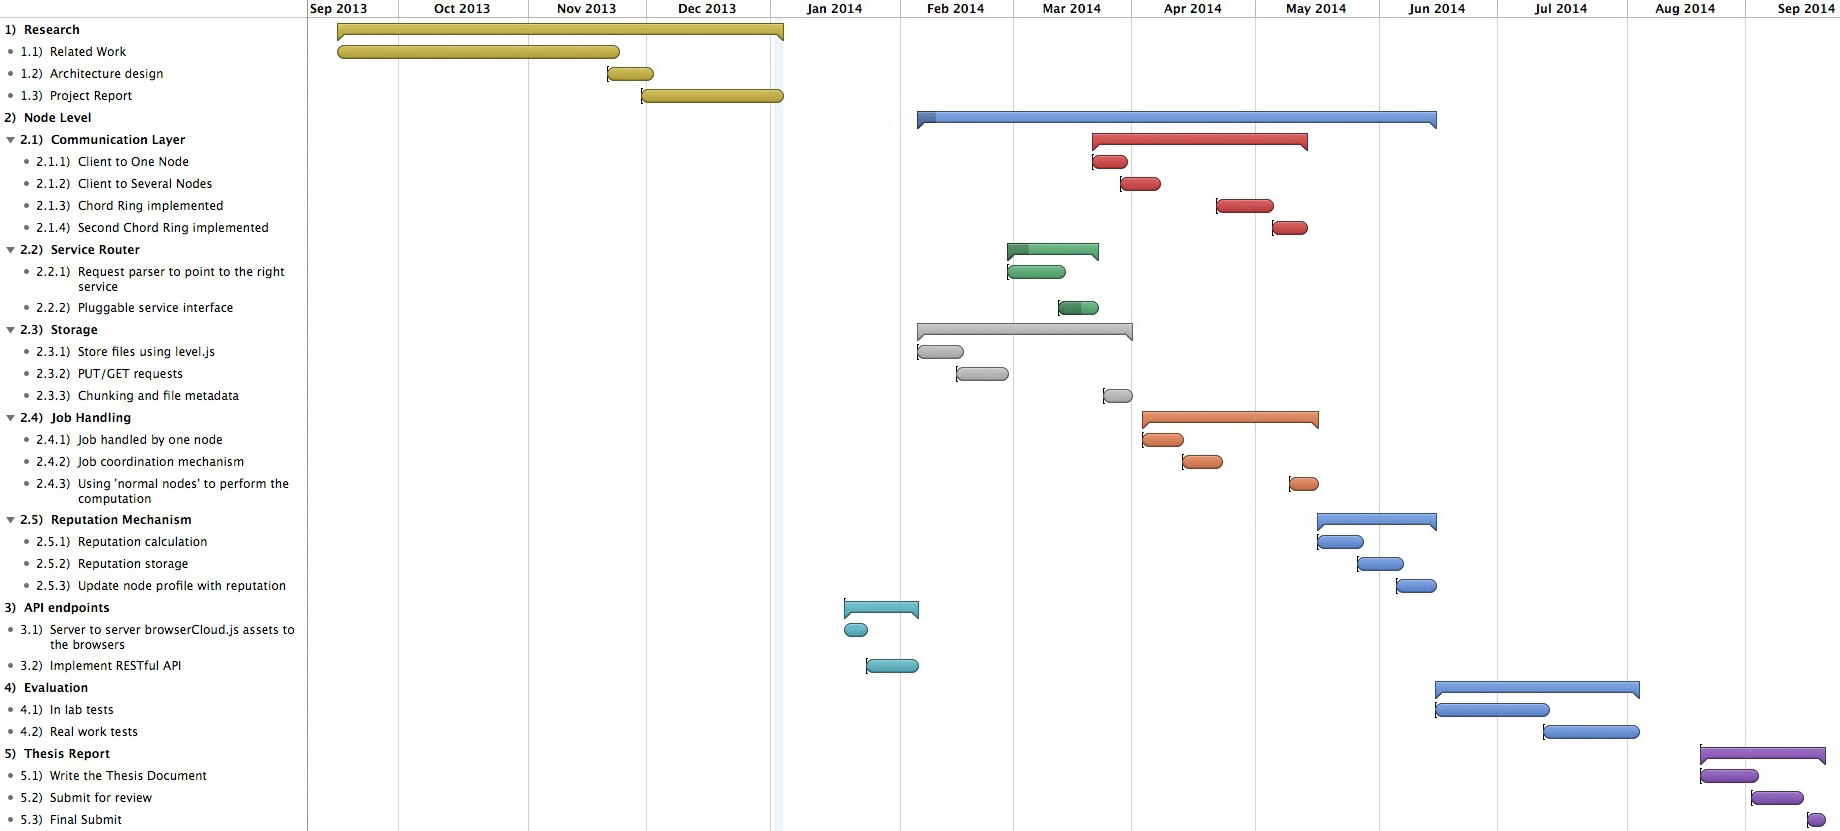
\includegraphics[angle=90,width=0.55\textwidth]{img/gantt.jpg}
  \caption{browserCloud.js development, evaluation and Thesis report schedule}
  \label{fig:gantt}
\end{figure}



\end{document}